\documentclass[final]{beamer}

\usepackage{amsmath}
\usepackage{amssymb}
\usepackage{amsthm}
\usepackage{booktabs}
% \usepackage[figurename=(c),labelsep=space]{caption} % Hack
\usepackage{enumitem}
\usepackage{float}
\usepackage{geometry}
\usepackage{mathtools}
\usepackage{microtype}
\usepackage{nicefrac}
\usepackage{physics}
\usepackage{siunitx}
\usepackage{tikz}
\usepackage{xcolor}
\usepackage{pgffor}
\usepackage[orientation=landscape,size=custom,height=28,width=30.48,scale=1.0]{beamerposter}
\usepackage{adjustbox}
\usepackage{subcaption}

\graphicspath{{figs/}}

\usepackage[sfdefault,semibold]{libertine} % a bit lighter than Times--no osf in math
% \usepackage[libertine,vvarbb]{newtxmath}
\usepackage{eulervm}
\usepackage[scr=esstix,cal=boondoxo]{mathalfa}

\usetikzlibrary{arrows, shapes.misc, positioning, fit, calc}
\tikzset{%
  invisible/.style={opacity=0,text opacity=0},
  visible on/.style={alt=#1{}{invisible}},
  alt/.code args={<#1>#2#3}{%
    \alt<#1>{\pgfkeysalso{#2}}{\pgfkeysalso{#3}} % \pgfkeysalso doesn't change the path
  },
}

\usecolortheme[snowy]{owl}
\usefonttheme{professionalfonts}
% \usefonttheme{serif}
\setbeamersize{text margin left=0pt, text margin right=0pt}
\setbeamertemplate{blocks}[rounded][shadow=true]
\setbeamercolor{title}{fg=white,bg=blue} % Temporary; tweak me!
% \setbeamercolor{block title}{bg=blue!70, fg=white}
\setbeamercolor{block title}{bg=blue, fg=white}
\setbeamercolor{block body}{bg=black!9}
\setbeamerfont{block title}{series=\bfseries}

% Hack a margin into blocks.
\newenvironment{mblock}[1]{%
  \begin{block}{#1}%
    \begin{adjustbox}{minipage=\linewidth-3ex, margin=1.5ex, center}}%
{\end{adjustbox}\end{block}}

% It's a hack, but it works.
\title{%
  \parbox{0.02\textwidth}{\hspace{-2.25ex}
\includegraphics[width=4.5ex]{nsf}\hfil}%
  \parbox{0.18\textwidth}{\small
    \textbf{Physics \textsc{Reu}: Summer 2020} \\
    Rensselaer Polytechnic Institute
  }
  \parbox{0.55\textwidth}{\Huge
    Understanding visual complexity with statistical physics
  }
  \parbox{0.20\textwidth}{\hfill
    Alex Striff \& Vincent Meunier
  }
}
\author{}
\date{}

\begin{document}
\begin{frame}[t]{}
  % \vspace{-8pt}
  % \begin{beamercolorbox}{}
  %   \maketitle
  % \end{beamercolorbox}
  % \vspace{-1.5in}
  \centering
  \tikzstyle{cclip}  = [transparent, circle, minimum size=5cm, outer sep=6pt]
  \tikzstyle{clabel} = [text opacity=1, inner sep=0pt, text=white, font=\bfseries]
  \begin{tikzpicture}[
    visible on=<+->,
    x=7cm,
    y=7cm,
    cclip/.style = {transparent, circle, minimum size=5cm, outer sep=6pt},
    clabel/.style = {text opacity=1, inner sep=0pt, text=white, font=\bfseries, align=center}
    ]
    \node[visible on=<.(14)->, circle, fill=black!10, inner sep=0pt,
      outer sep=0pt, minimum size=19cm]
      (visual world) at (0,0) {};
    \node[visible on=<.(14)->, below=of visual world, inner sep=0pt, outer sep=0pt, text
      width=21cm, align=center] {%
        \textcolor{green}{We} cannot \textcolor{red}{directly perceive} the
        true nature of the world, but we can form models to
        \textcolor{orange}{indirectly perceive} nature. A model must represent
        nature, while still being something we can readily look at and use to
        guide thought. \textbf{What are good models of how nature looks to
        us?}
      };
    \begin{scope}[visible on=<.->]
      \node[cclip] (natural) at (120:1) {};
      \clip (natural) circle (2.5cm)
      node {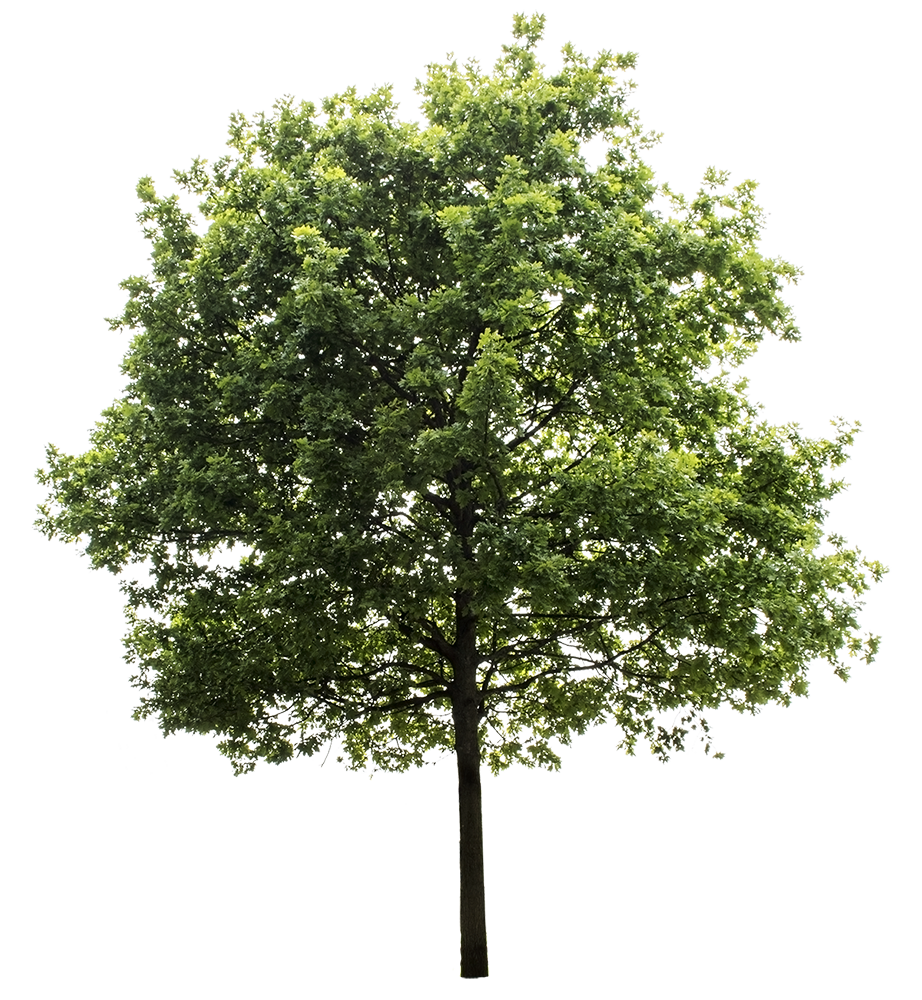
\includegraphics[width=5cm]{tree-natural}};
      \node[clabel] at (natural) {Natural};
    \end{scope}
    \begin{scope}[visible on=<.(1)->]
      \node[cclip] (seen) at (0,0) {};
      \clip (seen) circle (2.5cm)
      node {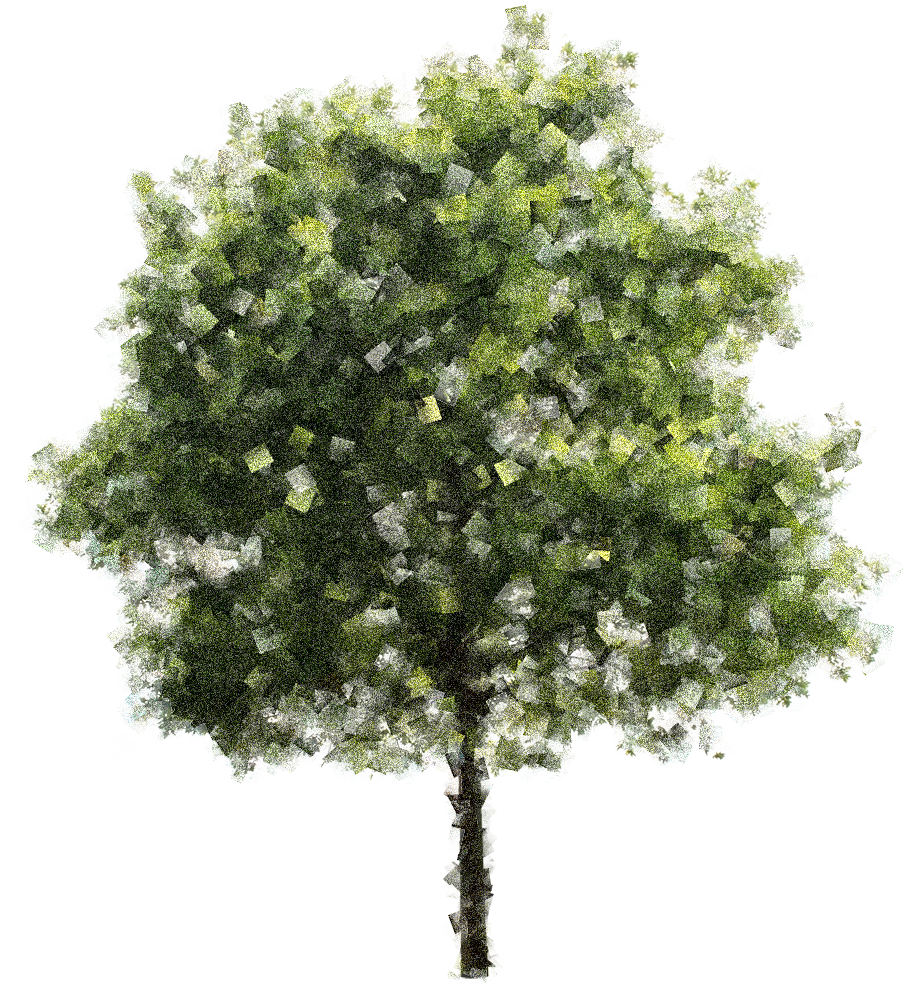
\includegraphics[width=5cm]{tree-seen}};
      \node[clabel] at (seen) {Sight};
    \end{scope}
    \begin{scope}[visible on=<.(2)->]
      \node[cclip] (cartoon) at (0:1) {};
      \clip (cartoon) circle (2.5cm)
      node {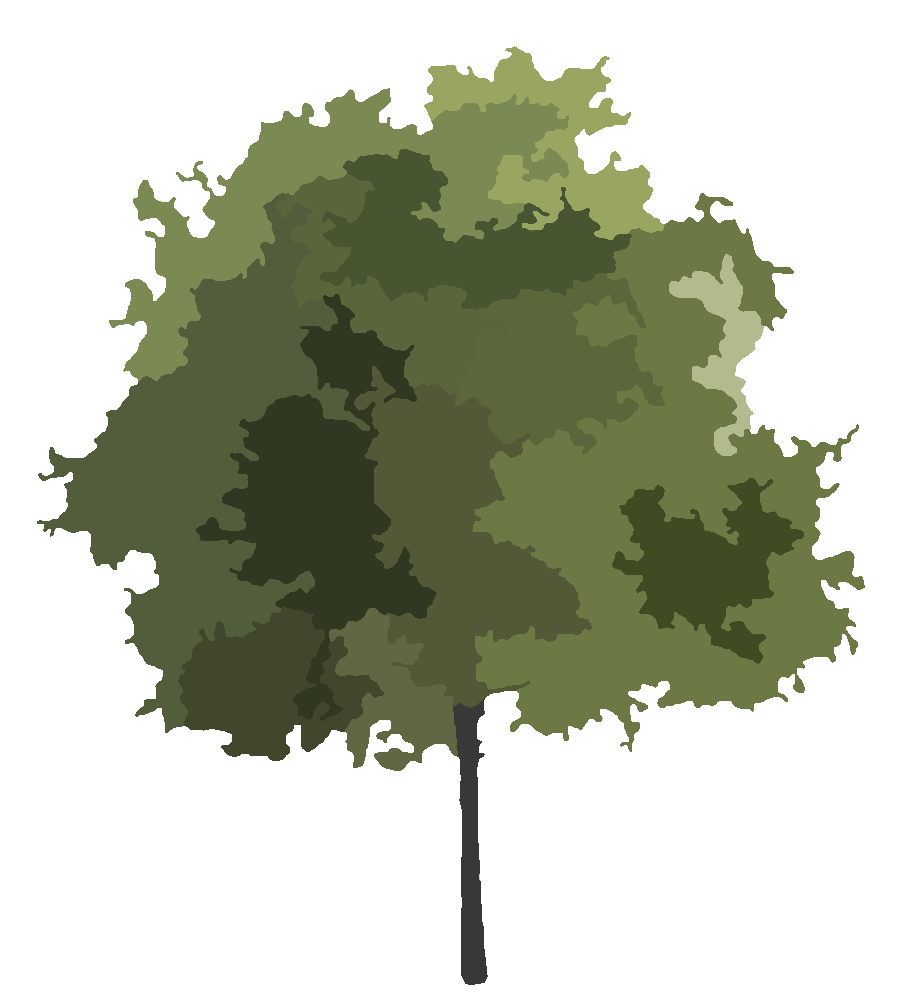
\includegraphics[width=5cm]{tree-cartoon}};
      \node[clabel] at (cartoon) {Thought};
    \end{scope}
    \begin{scope}[visible on=<.(7)->]
      \node[cclip] (bitmap) at (-120:1) {};
      \clip (bitmap) circle (2.5cm)
      node {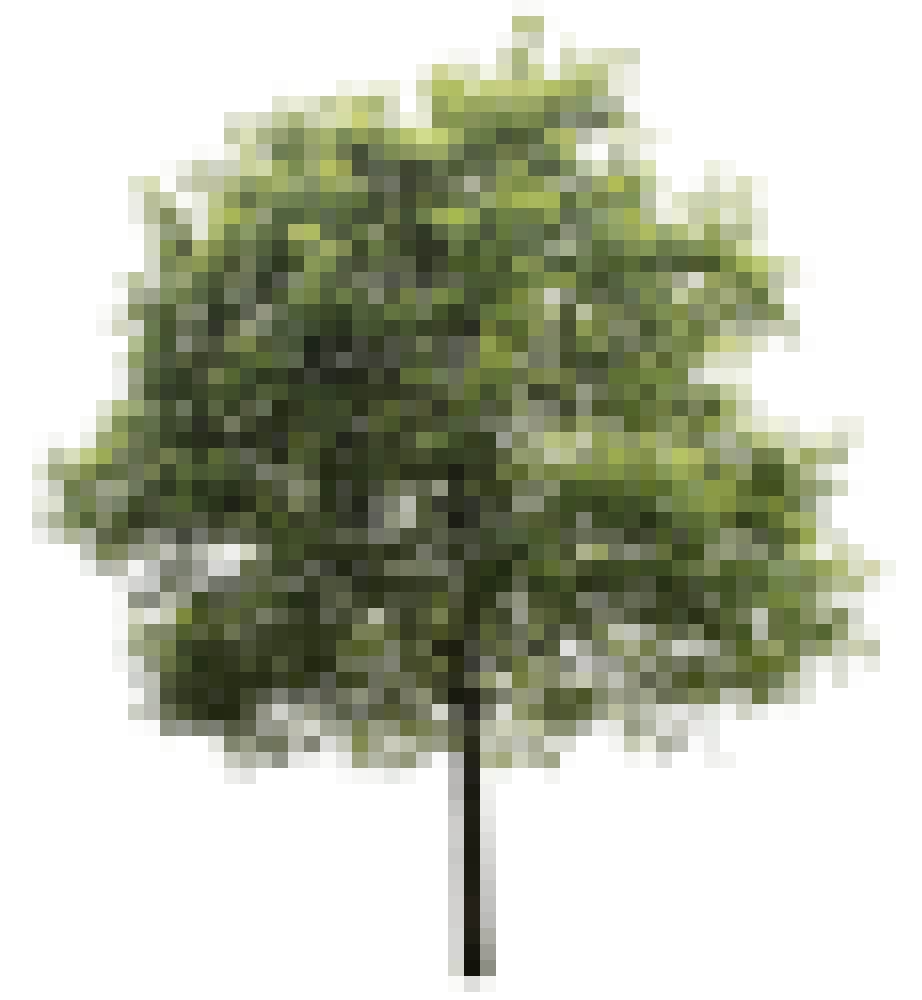
\includegraphics[width=5cm]{tree-bitmap}};
      \node[clabel] at (bitmap) {Model};
    \end{scope}
    \begin{scope}[->, line width=3pt]
      \begin{scope}[green]
        \draw[visible on=<.(1)->] (natural) to[bend right=15] node[below,sloped]{Look} (seen);
        \draw[visible on=<.(2)->] (seen) to[bend left=15] node[above]{Perceive} (cartoon);
        \draw[visible on=<.(3)->] (cartoon) to[bend left=15] node[below]{Reflect} (seen);
        \draw[visible on=<.(9)->] (bitmap) to[bend left=15] node[above,sloped]{Look} (seen);
      \end{scope}
      \begin{scope}[orange]
        \draw[visible on=<.(8)->] (natural) to[bend right=45] node[above,sloped,rotate=180]{Represent} (bitmap);
        \draw[visible on=<.(10)->] (seen) to[bend left=15] node[below,sloped]{Rep.} (bitmap);
        \draw[visible on=<.(11)->] (bitmap) to[bend right=45] node[above,sloped]{Learn} (cartoon);
        \draw[visible on=<.(12)->] (cartoon)  to[bend left=25] node[above,sloped]{Abstract} (bitmap);
        \draw[visible on=<.(13)->] (bitmap) to[bend left=25] node[above,sloped]{Generate} (natural);
      \end{scope}
      \begin{scope}[red]
        \draw[visible on=<.(4)->] (natural) to[bend left=25] node[above,sloped]{Omniscience} (cartoon);
        \draw[visible on=<.(5)->] (cartoon) to[bend right=45] node[above,sloped]{Physics} (natural);
        \draw[visible on=<.(6)->] (seen) to[bend right=15] node[above,sloped]{Psych.} (natural);
      \end{scope}
    \end{scope}
    \addtocounter{beamerpauses}{14}
  \end{tikzpicture}
\end{frame}
\end{document}

